 \documentclass[12pt,english]{article}
\usepackage[utf8]{inputenc}
\markright{Pearse et al.\hfill Assessing the Effects Imputation on ED Values\hfill}
\usepackage{geometry}
\geometry{verbose,letterpaper,tmargin=2.54cm,bmargin=2.54cm,lmargin=2.54cm,rmargin=2.54cm}
%\geometry{verbose,letterpaper,tmargin=.1cm,bmargin=.1cm,lmargin=.1cm,rmargin=.1cm}
\usepackage{graphicx}
\DeclareGraphicsExtensions{.pdf,.png,.jpg}
\usepackage{amssymb,amsmath}
\usepackage{epstopdf}
\usepackage{tocbibind}
\usepackage[toc,page]{appendix}
\usepackage{supertabular}
\DeclareGraphicsRule{.tif}{png}{.png}{`convert #1 `dirname #1`/`basename #1 .tif`.png}
\usepackage{url}
\usepackage{subcaption}
\usepackage{caption}
\usepackage[super]{nth}
\usepackage{lineno} \linenumbers
\usepackage[doublespacing]{setspace}
\usepackage[parfill]{parskip}
\setlength{\parindent}{0pt}
\usepackage[citestyle=authoryear,bibstyle=authoryear,sorting=nyt,maxcitenames=2,maxbibnames=10,minbibnames=6,doi=false,url=false,isbn=false,firstinits=true,uniquename=false,uniquelist=false]{biblatex}
\bibliography{edge_sims}
\renewbibmacro*{name:andothers}{% Based on name:andothers from biblatex.def
  \ifboolexpr{
    test {\ifnumequal{\value{listcount}}{\value{liststop}}}
    and
    test \ifmorenames
  }
    {\ifnumgreater{\value{liststop}}{1}
       {\finalandcomma}
       {}%
     \andothersdelim\bibstring[]{andothers}}
    {}}
\renewcommand*{\finalnamedelim}{%
  \ifnumgreater{\value{liststop}}{2}{\finalandcomma}{}%
  \addspace\&\space}
\renewbibmacro{in:}{}
\AtEveryBibitem{%
  \clearfield{day}%
  \clearfield{month}%
  \clearfield{endday}%
  \clearfield{endmonth}%
}
\DeclareFieldFormat[article]{citetitle}{#1}
\DeclareFieldFormat[article]{title}{#1}
\DeclareFieldFormat[article]{pages}{#1}
\DeclareNameAlias{sortname}{last-first}

\usepackage{changes}
\setdeletedmarkup{\textcolor{red}{\sout{#1}}}

\begin{document}
\setlength{\parindent}{0pt}
\section*{Title page}

\textbf{Article title}: Assessing the Effects Imputation on ED Values

\textbf{Running head}: Assessing the Effects Imputation on ED Values

\textbf{Authors:} K.\ Bodie Weedop$^{1}$, William D.\ Pearse$^{1}$\

$^1$ Department of Biology \& Ecology Center, Utah State University,
5305 Old Main Hill, Logan UT, 84322

$^*$To whom correspondence should be addressed:
\url{will.pearse@usu.edu} or \url{kbweedop@gmail.com}
% I'm doing this because your email might not be around forever,
% right? If you would prefer to put a Gmail address or something up
% here that would be fine. Typically, I prefer to have only one
% contact author, as it can make things a bit confusing otherwise.

\textbf{Word-count}: 5680 (abstract, main text, acknowledgements, and
  references)

\clearpage
\section*{Abstract}


\textbf{Keywords}: 

\clearpage
\section*{Introduction}
Evidence from the fossil record and present-day studies argue we are
in the midst of, or entering, a sixth mass extinction
\autocite{Barnosky2011, Ceballos2015}, such that more species than
ever are declining and/or in danger of extinction across a range of
environments \autocite{Wake2008,Thomas2004}. Habitat destruction
\autocite{Brooks2002}, invasive species \autocite{Molnar2008}, climate
change \autocite{Pounds2006}, and disease \autocite{Lips2006} are some
of the leading causes of species declines globally. Conservation
biologists seek\deleted{s} to \replaced{reverse}{overcome} these
declines and their detrimental effects on species populations\added{,
  but in reality they have limited resources with which to do
  so.}. \added{This challenge, termed the} \deleted{Even still,
  researchers and conservationists are confronted with }``Noah's Ark
problem'' \autocite{Weitzman1998}, \added{is the basis for modern
  conservation prioritisation and triage (XXX define
  triage).}\deleted{or an unfortunate reality of insufficient, finite
  resources to confront the increasing amount species requiring
  conservation effort.}

Conservation triage has provided an efficient decision making process
for allocating finite resources to obtain the greatest return
\autocite{Bottrill2008}. \added{A sentence about how triage requires
  decision-making, and so you need a metric to guide that decision
  process.}
% This is a good example of where you've got to lead the reader
% through, step-by-step, each of the concepts you're introducing
One of these triage strategies which have been introduced
and used most widely is \added{the} EDGE \added{metric}
\autocite[\added{Evolutionary Distinction and Globally
  Endangered;}][]{Isaac2007}. This method prioritizes species
according to two metrics: \replaced{E}{e}volutionary
Evolutio{D}{d}istinctiveness (ED) and \replaced{G}{g}lobal
\replaced{E}{e}ndangerment (GE). ED measures relative contributions to
phylogenetic diversity made by each species within a particular clade
\autocite{Isaac2007}. Such contributions are assessed by quantifying
the amount of branch length which is unique to each species within the
overall phylogeny. GE values are assessed by assigning numerical
values to each of the World Conservation Union (IUCN) Red List
Categories.
% Might be nice to mention and/or cite some of the discussion around
% how to assign these numerical values; e.g., Mooers et al. (2008)
As species become increasingly threatened and are placed
into more concerning categories (\replaced{}\emph{e.g.},}{e.g.} from
% Always do e.g. in italics and with a comma after it
Vulnerable to Endangered), the GE numerical value increases. Increases
in either ED or GE place a particular species at a higher priority for
conservation effort.

% Here's an idea for a middle paragraph that would serve as a bridge
% between this and the next: introduce some examples of the method
% being applied in the real world. It could have a structure a bit
% like this:
% * Statement that EDGE lists have been calcualted for a number of
% species (give examples)
% * State that there is some discussion in the literature about what
% the best kind of EDGE-like metric should be (cite HEDGE et al.).
% * There is also discussion in the literature about whether we should
% account for likelihood of success in conservation, relative cost of
% conservation interventions, and complementarity when designing our
% metrics. This gives you a nice place to cite the "other side" of the
% debate.
% * However, EDGE has formed the basis of a very successful
% program. State a few nice facts about it.
% * BUT the thing that's holding us back is missing data. Phylogenetic
% data is often missing, *and so is imputed* - cite the taxa and the
% studies that use imputation.
% ... this nicely leads into the next paragraph, where you talk about
% how imputation happens and why we need to understand it.

% Some of the text in this paragraph will now be pulled into the one
% above. You'll also find that you'll now be able to talk in a little
% bit more detail about *how* imputation takes place, citing the Kuhn
% polytomy paper and the Jetz paper, I suppose. Does that make sense?
In the event of missing DNA or trait data, species are often difficult
or not able to be placed onto a phylogeny. Even in the face of such
uncertainty and missing data, it is understandable that conservation
biologists want to make prioritizations. However, if we are using a
quantitative method for prioritizing species, we should remain
consistent even when uncertainty arises. To our knowledge, a proper
and efficient method for prioritizing species where there is missing
data is still untested. This issue pertains mainly to the calculation
of ED than GE. The IUCN has collected data on most major clades, and
has a strategy for assigning Red Listing values these species which we
know little information and are considered Data Deficient (DD). IUCN
and other conservation organizations support focus on DD species just
the same as Critically Endangered and Endangered species to ensure
consistency \autocite{Rodrigues2006}. The major area of uncertainty in
phylogenetic prioritisation is phylogenetic data. In the past, missing
species data and poorly resolved trees have been addressed using
imputation \autocite{Collen2011, Isaac2012, Jetz2014}. However, to our
knowledge, there has been no systematic investigation of the efficacy
of such imputation, both in terms of the accuracy with which imputed
ED values are estimated, and the effect on other known species'
scores. Indeed, it is unclear whether any significant information on
ED is gained by imputing species which cannot be placed on the
phylogeny. It is also not well understood how simply removing missing
species, compared to performing imputation, would effect ED values. It
may be that simply excluding missing species may be less intrusive
than imputation. In searching for a solution for missing species, we
may be negatively affecting correct ED values and disrupting EDGE
rankings in the process. As the desire to use ED and phylogenies for
conservation triage grows, the importance of such tests and a
consensus on how to resolve cases of phylogenetic uncertainty becomes
more urgent.

% This is a bit short - you can give a bit more detail and "big up"
% the paper a little. I've given some guides below, but you can fill
% in from there I sense.
\added{Here we assess the extent to which EDGE rankings based upon
  imputed phylogenies can be used within applied conservation
  biology. To do this, we use an imputation approach...} \deleted{Here, we
assess and compare the impact that missing species versus phylogenetic
imputation has upon ED values.} In doing so, we hope to understand the
effect that both methods have on ED values and offer a viable solution
for dealing with missing data species. Missing species were simulated
and removed from trees in two ways: randomly and in a phylogenetically
biased manner. Additionally, we tested how ED values were affected by
resolving and imputing polytomies of varying sizes on a phylogeny. We
found that ED values are by removing missing species. Here is a
reference to figure.

\section*{Methods}
\replaced{Here we use a simulation approach to test the effect of
  removing and imputing species on a phylogeny on subsequent ED
  (Evolutionary Distinctiveness) scores of species.}{We attempted to
  demonstrate the effects of removing or imputing species which cannot
  be placed onto a phylogeny.}
% Don't attempt to do something, do it!
\replaced{Since empirical studies do not (to our knowledge) impute GE
  (Global Endangerment) scores for species, and our focus here is on
  the importance of phylogenetic structure, we focus on the impact of
  imputing ED values.}{While assessing the impact of dropping species
  and phylogenetic imputations, we were primarily focused on ED
  values. In testing the effects on these values, we remain focused
  upon ED as a single variable.}
% Then go on to explain that EDGE is ED + GE (...well, technically
% times GE, but still...) and that any imputation that uses real GE
% values as well with have pseudo-precision. This is an important
% point, and we want to bring it up now because it will matter in the
% discussion also.
\deleted{We exclude GE because it would only add complexity while not
  providing any additional information to our particular
  investigation.}
% State *WHY* it would do that. People won't just believe you, and
% they need to know why.

\deleted{In each test, we simulated 100 phylogenetic trees and
  manipulated each tree's tips or clade.} All simulations\deleted{,
  calculations,} and analyses were performed using R
\added{\autocite[version 3.4.0;][]{R2017}}. \added{For each
  combination of parameter values in a simulation, we performed 100
  replicate simulations.} Original and manipulated trees were
simulated under a pure-birth Yule model using the
\replaced{\texttt{sim.bdtree}}{sim.bdtree} function
\replaced{\texttt{geiger}}{`geiger'} R package
\autocite{Harmon2007}.
% The next three sentences are too vague. Be explicit: this is the
% simplest model possible (state what it represents/is), thus anything
% that doesn't work on this shouldn't have a hope in hell of working
% in a more complex biological simulation. We're setting up the best
% possible case by imputing under the exact model that the data were
% simulated under in the first place - in empirical studies, you would
% have to estimate this model.
This particular model was chosen to maintain simplicity. Results from
this simple model should be applicable to other more complex
scenarios. Also, to reduce uncertainty, we used the same model
throughout each of the simulations. In reality, we would be estimating
the parameters of the model which the phylogeny is built upon. The
function \replaced{\texttt{ed.calc}}{ed.calc} within the R package
\replaced{\texttt{caper}}{`caper'} was used to calculate ED values for
each tree \autocite{Orme2013}.

% You should only be putting details in this section that you did for
% every one of the methods. You didn't do this for every single
% simulation type, so don't report it here. This should be worked into
% the next section.
\deleted{We assessed the impact that removing missing species has upon
  ED values using the correlation of all ED values for the tips
  remaining within both trees. To evaluate the effect that imputation
  has upon ED values, we calculated ED for all tips in both the
  original and manipulated trees while excluding the focal clade where
  imputation has occurred. These ED values were compared using a
  correlation. Additionally, we did the same calculations and
  comparison using only the original focal clade and its' simulated
  replacement. If missing species have no effect upon ED values, we
  expect a high, positive correlation coefficient between the original
  tree and its' manipulated counterpart.}

\subsection*{Assessing the impact of missing species on EDGE-listing}
\added{Our first set of simulations assesses the impact that species
  missing from a phylogeny have on estimated ED scores. If, when
  species are missing from a tree, the ED scores of the remaining
  species in the tree are XXX this implies XXX.}
% Fill in the blank above to justify the rationale behind this section
If missing species has a negative effect on ED values
% What does "negative effect" mean? Be more precise.
, then the correlation between the ED of the species in the original
tree and the same tree with a fraction of tips removed in some manner
should be significantly different from 1. \added{We performed
  simulations on phylogenies of different sizes (number of taxa: XXX,
  XXX), removing constant fractions of tips from the tree (0\%, 1\%,
  2\%, ..., 19\%, 20\%).}
% What did you do if the percentages were non-integers? Did you round
% the numbers?...
\deleted{To investigate the degree of this effect, we removed tips
  from simulated trees (Number of taxa = 64, 128, 256, 512, 1024,
  2048, 4096) at random and by phylogenetic clusters. To assess the
  effect under varying amounts of uncertainty, fractions of tips
  dropped ranged from 0 to 0.2 of total tree tips.}

% A sentence saying why you did both random species loss and
% phylogenetically-biased species loss. What biological process is
% this supposed to simulate?...
Missing species at random was simulated by selecting species at random
without replacing, and removing those species from the tree. This
randomization had no regard for phylogenetic structure. Missing
species related by some character trait was tested by simulating
character trait values for each tip. These simulations were all
performed under a constant rate Brownian-motion model
(\replaced{$\sigma^2$=0.5}{par = 0.5}, starting root value = 1).
% Do you need to repeat this with different sigma values? Also, this
% parameter is sigma squared, right?
% Re-write the next two sentences - be specific the first time you
% state it.
Tips were dropped if their character trait values place them into the
upper quantile which had been selected to be dropped. More
specifically, if the fraction to be dropped was 0.1, species within
the 90th quantile of character trait values are dropped. This is
equivalent to Felsenstein's threshold model \autocite{Felsenstein2004}
% Was this paper really written by Felsenstein and his brother? His
% brother is a computer scientist...
\added{state why this model is a useful one---re-state the propoerty
  it has, linking it back to why this is a useful set of simulations
  to be doing}.

\subsection*{Assessing the impact of phylogenetic imputations}
We tested the impact of imputing missing species onto a clade of a
particular size (sizes \replaced{3, 4, 5, ..., 30, 31, 32}{3 through
  32}) which originated from a tree of a particular size
(\replaced{N}{n}umber of taxa = 64, 128, 256, 512, 1024).
% Why do you keep capitalising words? I'm asking seriously - there's
% probably a reason for it, I just don't know what it is
To simulate the effect that phylogenetic imputation has upon these
simulated trees, we randomly chose clades within each tree and treated
it as a polytomy to be resolved.
% That might be how we did it in the code, but it's not necessary to
% write in the methods that we treated the clade as a polytomy
The clade selected was removed from the original tree and a new
separate tree of the same size was simulated under the pure-birth
model used before and placed back where the original clade was
removed. \added{Thus we have imputed each clade under the same model
  used to generate it. In an empirical study, this would be done
  by... and so our method is being generous because...} By doing this
, we replicated the process of imputation of a clade which has been
resolved. \deleted{To ensure that this is representative of cases
  where imputation is used, 100 repetitions of this simulation were
  performed across different parameter settings.}
% That wasn't why we did it 100 times...

\added{To assess whether clades, once imputed, had similar ED scores,
  we ... We also looked at ranks, because... We statistically modelled
  these as a function of ..., hypothesising that each would matter
  because...}

\section*{Results}
% I like that you've matched the sub-headings of the methods onto the
% results, but I've gotten rid of them in this case because the first
% section is essentially two sentences and it feels odd to have a two
% sentence section. I applaud the logic in keeping the structure,
% though.

%\subsection*{Assessing the impact of missing species on
%    EDGE-listing}

\replaced{While the random loss of species from a phylogeny does not
  appear to affect the ED values of the remaining species,
  phylogenetically-patterned loss does (Fig.\ \ref{randomVsClustered}
  and Table \ref{XXX}). Under both random and phylogenetically
  patterned loss, XXX increases with XXX, although the effect is much
  more extreme (XXX times; Table \ref{XXX}) for XXX.}{ED values for
  remaining species were significantly affected by the fraction of
  species which were removed (Table 1). However, different effects are
  seen when dropping species at random and in clustered manner
  (Fig. \ref{randomVsClustered}). Dropping species at random has a
  reduced effect when compared to the effect which dropping species in
  a clustered manner has on remaining ED values
  (Fig. \ref{randomVsClustered}).}
% You've written this backwards, in that you state the result at the
% end of the paragraph. You also are slipping into a very passive-y
% description of the results here.

\section*{Results}
\subsection*{Assessing the impact of missing species on EDGE-listing}

Our results demonstrate that the comparison between ED values before and after
species were removed was negatively affected by the fraction of species removed
in both treatments (Table 1). Similar but slightly different effects are seen
when dropping species at random and in clustered manner (Fig.
\ref{randomVsClustered}). Interestingly, the rate at which ED values deviate
from their true value is increased with species missing at random. 

\begin{figure}[!ht]
  \center
  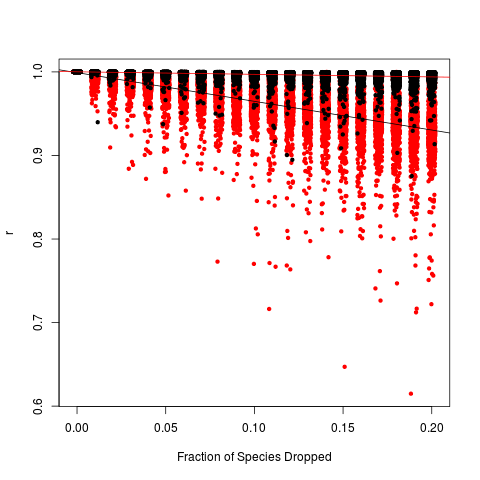
\includegraphics[width=.5\textwidth]{randomVsCluster.png}
  \caption{\textbf{R-values plotted against the fraction of species dropped at
  random versus clustered manner.} The color of data points denote whether
  species were dropped at random (orange; n = 100) or in clustered manner
  (grey; n = 100). The regression lines are demonstrating the relationship when
  species are dropped at random (red) and in a clustered manner (clustered). The
  correlations represent a comparison of the ED values (before and after
  species are dropped) of species which remain on the on the phylogeny after
  other species are dropped. 
  }
  \label{randomVsClustered}
\end{figure}

\begin{table}[ht]
  \centering
  \begin{tabular}{rrrrr}
    \hline
      & Estimate & Std. Error & t value & Pr($>$$|$t$|$) \\
      \hline
      (Intercept) & 1.0315 & 0.0013 & 821.39 & $<$0.0001 \\
      Fraction of Species Dropped & -0.4696 & 0.0020 & -233.16 & $<$0.0001 \\
      Random Treatment & 0.0630 & 0.0018 & 35.47 & $<$0.0001 \\
      Number of Species Overall & 0.0000 & 0.0000 & 7.89 & $<$0.0001 \\
      Fraction of Species Dropped:Random Treatment & -0.2774 & 0.0028 & -97.45 & $<$0.0001 \\
      Random Treatment:Number of Species Overall & 0.0000 & 0.0000 & -4.38 & $<$0.0001 \\
      \hline
    \hline
  \end{tabular}
\caption*{\textbf{Table 1: ANCOVA model summary describing the effect of
dropping species on remaining species ED Values.} The fraction of species
dropped significantly affects the the remaining ED values. Dropping the
fraction both at random and in clustered manner both have negative effects on
the remaining ED values ($F_{139696, 5}$ = 40350, $R^{2}$ = 0.5908,
p$<$0.0001).}
\end{table}

% \subsection*{Assessing the impact of phylogenetic
% imputations}

\added{We find no support for a correlation between the imputed and
  true ED values for a species within an imputed clade (Fig.\
  \ref{imputationTrend}, table XXX). We do find evidence that, when
  imputing larger clades, the variation in the correlation is lesser
  (quantile regression), but this could be due to XXX.} \deleted{ED
  values for the full tree while excluding the focal clade remain at
  1 and unaffected. However, ED values for the imputed clades are
  significantly affected by the use of imputation. As the size of
  the focal clade increases, the informative value of the ED values
  within the clade decreases (Fig. \ref{imputationTrend}). However,
  even when imputing smaller clades, ED values did not regularly
  reflect the true ED values (Table 2).} \replaced{We found}{Our
  analysis demonstrates} that measures of the
\replaced{true}{original} phylogeny such as phylogentic diversity
(PD), lambda, Colless' Index, skew, and kurtosis do not provide any
indication that imputation would negatively affect ED values
(Appendix A). \deleted{Additionally, j}Just as imputed ED values did
not reflect true ED values, the rankings of species within the focal
clade were altered significantly \added{under imputation}
(Fig. \ref{rankingError}; Table XXX). Our model suggests that with
increases in the size of the imputed clade and overall number of
species, species within the clade are ranked farther from their true
ranking (Table 3). \replaced{For example}{More specifically}, our
% I replaced this because, technically, your example isn't really
% more specific, rather it's an example, if that makes sense?
model suggests that by imputing a clade of three species within a
phylogeny of 128 species, the species within the clade would be 60
rankings from their true rank on average.
% You've got to back this up with a reference to the appendix (maybe
% that's what your next sentence does). If you're going to make
% reference to this, highlight that this is interesting in the context
% of your first set of results: this is a phylogenetically biased
% thing that you've done, and so imputation has corrected for the
% concern above (that phylogenetically biased loss of species is
% affected ED rankings in the remaining species). It has, however,
% given you some rankings for some species that were wrong. Make
% sense?
ED values outside of the focal clade were not affected by imputation.
% I don't understand what the sentence below means
While ED values within the focal clades were affected exclusively by
imputation, a notable error rate in ranking crucial species correctly
is present (Appendix B).

\begin{figure}[!ht]
  \center
  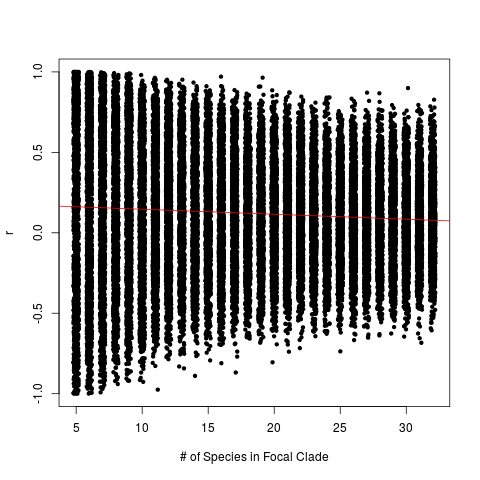
\includegraphics[width=.5\textwidth]{edModel.png}
  \caption{\textbf{R-values plotted against the number of species at focal
  clade.} Each data point denotes a correlative comparison between ED values
  within the focal clades where imputation has occurred. The regression line
  (red) and trend even closer to zero demonstrates the decrease in informative
  value of the imputed ED values. This is reinforced by the visual narrowing of
  r-values around zero.}
  \label{imputationTrend}
\end{figure}

\begin{table}[ht] 
\centering
\begin{tabular}{rrrrr}
  \hline
  & Estimate & Std. Error & t value & Pr($>$$|$t$|$) \\
   \hline
 (Intercept) & 0.1852 & 0.0533 & 3.47 & 0.0005 \\
   Size of Focal Clade & -0.0034 & 0.0002 & -16.56 & 0.0000 \\
   Size of Phylogeny & -0.0001 & 0.0001 & -0.41 & 0.6855 \\
   PD & 0.0001 & 0.0001 & 0.37 & 0.7108 \\
   Lambda & -0.0012 & 0.0524 & -0.02 & 0.9812 \\
   Colless' Index & 0.0016 & 0.0022 & 0.72 & 0.4687 \\
   Skew & 0.0043 & 0.0088 & 0.48 & 0.6288 \\
   Kurtosis & -0.0005 & 0.0009 & -0.63 & 0.5269 \\
   \hline
   \hline
\end{tabular}
\caption*{\textbf{Table 2: Effect of Clade Size on Imputed ED Values.} The
intercept describes that the correlation between the true and imputed values
begins quite low. As the clade size increases, this correlation only tends
toward zero. The total number of species in the full phylogeny along with
measures of the true phylogenetic diversity, lambda, Colless' Index, skew, and
kurtosis show no significant effect. ($F_{47992, 7}$ = 39.57, $R^{2}$ = 0.006,
p$<$0.0001).}
\end{table}

\begin{figure}[!ht]
  \center
  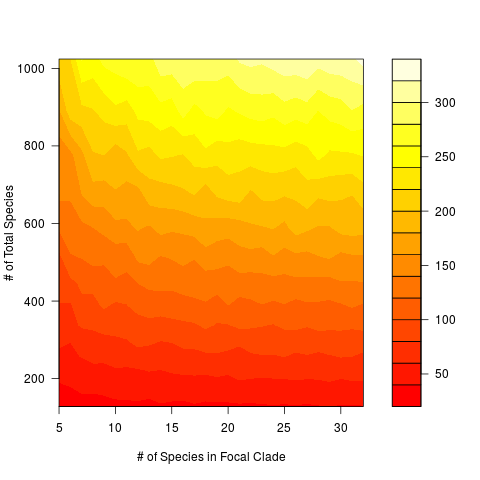
\includegraphics[width=.5\textwidth]{rankingError.png}
  \caption{\textbf{Mean ranking error of species within the focal clade.} The 
  gradient on the right demonstrates average number of posistions within the 
  full ranking that focal clade species shifted from their true rank.
  While controlling for the size of the full phylogeny and focal clade, species 
  within the focal clade were, on average, ranked far from the true rank. }
  \label{rankingError}
\end{figure}

\begin{table}[ht]
  \centering
  \begin{tabular}{rrrrr}
    \hline
   & Estimate & Std. Error & t value & Pr($>$$|$t$|$) \\
    \hline
  (Intercept) & -1.6344 & 0.0332 & -49.29 & 0.0001 \\
    Size of Focal Clade & 0.0900 & 0.0010 & 91.22 & 0.0001 \\
    Size of Phylogeny & 0.5179 & 0.0013 & 383.99 & 0.0001 \\
     \hline
     \hline
  \end{tabular}
  \caption*{\textbf{Table 3: Effect of Clade Size and Total Species on Ranking
  Error.} Model demonstrating the relationship between focal clade species
  ranking error and the size of imputed clade and overall phylogeny. Square-root
  transformations have been applied to both ranking error and size of phylogeny.
  Significant increases ranking error are seen when increasing sizes of both the
  imputed clade and phylogeny ($F_{47997, 2}$ = 77890, $R^{2}$ = 0.7644,
  p$<$0.0001).}
  \end{table}

\clearpage
\section*{Discussion}
% This opening paragraph reads a bit undergrad-report-y. Maybe
% re-structure it a bit like this:
% 1. General statement about phylogenetic prioritisation as an
% emerging tool (cites)
% 2. General statement about the dangers of uncertainty in any
% prioritization. State our aim: to understand how such uncertainty
% might affect prioritization.
% 3. List the two main take-homes (the bit with "our results
% demonstrate that...").
% ...while I'm here, some other comments I would make are (1) avoid
% using numbers for things unless you absolutely have to, because it's
% a bit jarring to read. (2) if you are going to use numbers, make
% sure they're consistent: (1) is better than 1), in my opinion, but
% using (1 and 2) as you do below makes it look like you're opening
% parentheses (as it did when I did just then).
Phylogenetic uncertainty and missing species are complications commonly
encountered when applying ED for prioritization \autocite{Isaac2007}. The aims
of our investigation were to (1 determine how removing missing species from a
phylogeny affects ED values for the remaining species and (2 demonstrate how
imputation affects ED values of species where imputation is performed. Our
results demonstrate that (1 missing a proportion of overall species both at
random and in a phylogenetic-biased manner have different yet significant
affects on remaining ED values throughout the tree and 2) imputation does not
recover the ED value or ED rank of an imputed species.

% I've moved this paragraph up here, so that the caveats come just
% after this intro paragraph. I've done this mostly because I want to
% add sections to the discussion, and I think it would be weird to
% have a section with a single paragraph.
\added{[Moved; see comments]} \replaced{Our results are derived solely
  from simulations under a simple model of diversification---the Yule
  model. We do acknowledge that, in the real world, lineages evolve in
  more complex ways than are captured by such a simple model.}{We
  acknowledge that a Yule model of evolution is a simple model and
  more complex models may be present in empirical data}.
% Technically, a model isn't present in empirical data: a model is
% something we fit to data. Biological processes can be more complex,
% if that makes sense?
While we do not have empirical data, our simulations are performed
under the same evolutionary model and therefore able to generalize for
more complicated cases which might be seen in empirical data.
However, our results demonstrate that even under a simple model
imputing species lead to a misrepresentation of true ED values.  Also,
we have not been given any implication through this investigation that
a more complex model would give any different results.
% You sort of phrase this backwards: state that even under this
% simplest model, and so one would think it would be the simplest to
% impute. Further, add that we can't think how a more complex model
% would help. Then state that, given this, we feel our results are
% likely to generalise from the simplest case to the more complex.
Nomrally, imputation is averaged across all numerous trees to get the
closest estimate of true ED values. However, imputed trees still
deviate from the true trees and therefore the average would also be
far from the true average.
% Describe in a single sentence how imputation takes place across the
% posterior distribution of trees. Point out that our results show
% there is uncertainty in that distribution of trees, which is our
% focus.

% You need to talk about why we didn't simulate GE scores on the
% phylogenies here.

\subsection*{\added{Uncertainty in imputed species}}
%...or some similar title - just something to break it up a bit
Missing species and poor phylogenetic resolution have been identified as causes
of uncertainty when calculating ED \autocite{Isaac2007}. Prior to our
investigation, we could not find any assessment of how missing species might
affect ED values of species which are not missing.
% Find a paper that talks about how missing species might affect it,
% cite that, and then say that they don't explicitly model or test
% what we are testing. That's a stronger way of framing things than
% saying "we can't find anything", because it shows you have read the
% literature and looked.
Our results demonstrate that \replaced{it matters not just how many
  species are missing from a phylogeny when calculating an EDGE score,
  but also how those missing species are distributed across the
  phylogeny}{missing species at random or in a phylogenetically-biased
  manner can have different effects on ED values
  \ref{randomVsClustered}}.
% Does it? The curves are very similar to me. See my comment below: if
% you give something quantitative, it's going to be easier for the
% reader to do something with this.
Both manners of missing species cause ED values of species easily
placed on the phylogeny to stray from their true values (Table
1).
% Don't use words like "stray"; report some kind of quantitative value
% as to how bad the effect is.
\deleted{Missing species at random} However, the manner (either
randomly or phylogenetically-patterned) in which species are missing
from the phylogeny is, to our knowledge, not normally investigated
when deciding how to address them. In light of our results, this
should be a concern when deciding how to move forward with missing
species.
% This is vague. Tell the reader *why* it should be a concern, and
% what they should do differently as a result.
We realize that we have provided just two ways in which
species could be missing from a phylogeny and there are more that
could occur. Missing species could be biased by some phylogenetic
pattern other than Brownian motion evolution. Nevertheless, our
investigation shows that missing species cause ED values of species
remaining in the phylogeny to deviate from the true value.
% I would frame this in exactly the same way as you should frame the
% Yule model thing. Say, yes, we realise this is a simple model, but
% it shows an effect, and so this is something to think about. I would
% speculate about the kind of model that would be interesting to look
% at further: perhaps one where species radiate in situ and stay in
% place. Thus you could be missing an entire clade and it would be in
% the same place. Maybe find some literature about how species tend to
% be missing from conservation prioritisation or phylogenies and then
% cite that. Just a few sentence of waffle, informed by the
% literature.

In the past, we have included missing species into the EDGE framework using
different methods. Collen et al. assigned the mean ED score of presumed
congeneric species to the missing species \citeyear{Collen2011}. More
frequently, missing species and poorly resolved clades have been dealt with by
imputing the missing species and assigning all the species of the resolved
clade the mean ED value obtained from all possible or numerous resolutions of
the clade \autocite{Isaac2007; Isaac2012}. This method has been adapted by
others and applied where there were large percentages (~30\%) of species
missing \autocite{Jetz2014}.
% I would give the actual number as well as the percentage; that will
% give people an idea of the scale of the problem.
% 30% of species doesn't sound too bad, in some ways, but ~3000 species does, if you follow my drift?
While imputation does include missing species, research has shown
imputed phylogenetic data leads to biases in some ensuing analyses
\autocite{Rabosky2014}.
% You're being a bit vague again. Rabosky has some quite specific
% take-homes: report them.
When considering the analysis of ED, our results show that imputation
does not recover true ED values nor ED rank of missing species
\ref{imputationTrend; rankingError}. Additionally, as the size of the
imputed clade increases, ED values within the clade stray, on average,
further from their true values.
% That word again! Cats and dogs are stray; I don't think an ED value
% can be :D
Even though we are including missing species into calculating ED, we
are not obtaining accurate information about those species. While
being uninformative, these ED values would lead to mispriortizing
species based on our results \ref{rankingError}.
% Be specific and quote some quantitative information.
Analyzing the performance of imputation of a clade less than five
species was not performed due to limitations of statistical validity
\autocite{Crawley2012}.
% this is also vague, and makes it all sound a bit fishy. You can turn
% this into a point of strength, something like:
% * We do not report correlations when the clades were smaller than 5,
%   because we can't report a correlation reliably with so little data
% * But, it would be surprising if our trend suddenly changed such
%   that, when imputing only one species, it did better.
% * Invoke Arne's 'the clade should have an average ED' argument to
%   support this. In smaller clades (i.e., two species, and you don't
%   know where that species goes) then you should just be sampling from
%   the prior. That prior is exponential, and so there's absolutely no
%   reason to suppose it will do any better than what we have
%   already. This is a more complicated argument, so have a bash at it
%   and then we can talk.

Even so, our results provide no indication
that the effects of imputation seen in our results would improve when
applied at smaller clades.

\subsection*{\added{Guidelines for the use of imputation}}
\replaced{We suggest there is a straightforward synthesis of these
  results that should be useful in applied conservation
  biology.}{Combining the previous arguments provides an interesting
  case of when imputation could be useful.} Both random and
phylogenetically-patterned loss of species affect ED values throughout
the tree. However, we found that ED values of non-missing species
remain relatively constant under imputation. Therefore, imputation
provides an interesting solution to missing species biasing ED values
of non-missing species.
% I don't think you mean interesting. Be *precise*: what does it give
% us? What doesn't it give us?
We have shown that imputing missing species would not provide accurate
ED values for missing species. However, it would provide a method of
avoiding the loss of species affecting ED values throughout the
remainder of the tree. Basing conservation priorities upon the ED
values of imputed species would lead to inaccurate
prioritization. Nevertheless, imputation may be useful to stop missing
species from biasing species easily placed on the phylogeny.
% Make sure you reference the *result* that you have found - that the
% correlation of the non-imputed species is high. You could even
% explicitly compare it with the correlation when there's no
% imputation: if the correlation is better, good news! It's given us
% something. If it's not... well, we can worry about that if you find
% it :D

Given these results, we \replaced{now present}{have developed several}
guidelines for how missing species should be dealt with and when
imputation might be appropriate when calculating EDGE. In the event of
missing species, we should be investigating the amount of species that
are missing and consider whether imputation is necessary.
% Your use of 'we' is confusing here; I sense you mean 'we the field
% of conservation biology', but you need to be more explicit. Also,
% "consider whether imputation is necessary" sounds a bit vague. Lay
% out for the reader that you're about to tell them when it is(n't)
% necessary.
For some context, in our analysis we found that if 30\% of species
are missing at random or in a phylogenetic-biased manner from the phylogeny,
respectively, ~80\% and ~89\% of the remaining ED values remained accurate.
% Is this what an r2 of ED values mean? I'm not quite sure that's
% exactly what an r2 means
Therefore if species are missing, we should verify that the amount of missing
species does not exceed a percentage which we have found to provide poor ED
values for remaining species. While below an acceptable percentage of missing
species, EDGE should be carried out without attempting to impute the
missing species.
% This could be a very good idea; are you saying to see if the
% fraction you're missing is greater than the error that would be
% added in? Check what I'm saying about the r2, but it sounds like you
% could have found a very nice rule of thumb. I would even consider
% using the phrase "rule of thumb", as it will drive home to the
% reader that you're giving a guide to thought.
However, if a larger proportion of species are missing, imputation may
be used but with some caution. ED values for species easily placed on
the phylogeny are relatively unaffected and can be trusted when
setting conservation priorities. Nevertheless, ED values and ranks of
species which have been imputed should either be ignored or used
cautiously within EDGE.
% Bring in something quantitative here as well - reference the average
% error in ranking, and use that to give another 'rule of thumb' as to
% how variable the ranking could be for a species with no data. Does
% that make sense?
By following these guidelines we avoid biasing species which are
easily placed on the phylogeny even in the event that imputation is
used.

\section*{Acknowledgments}

\clearpage
\printbibliography

\clearpage
\appendix
\section*{A. Effect of Measures of the True, Full Phylogenies}

\begin{figure}[!ht]
  \center
  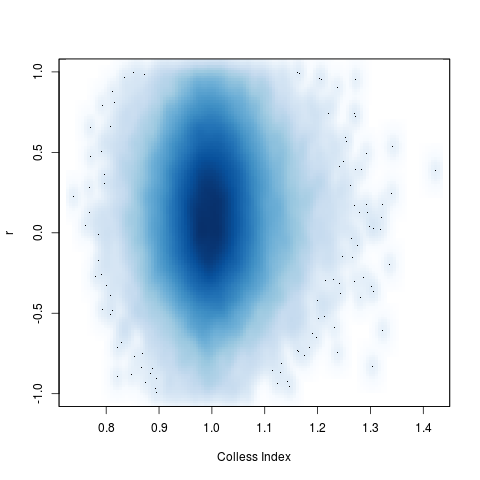
\includegraphics[width=.5\textwidth]{trueColless.png}
  \caption{\textbf{Effect of the True Colless Index of FullPhylogeny.}}
\end{figure}

\begin{figure}[!ht]
  \center
  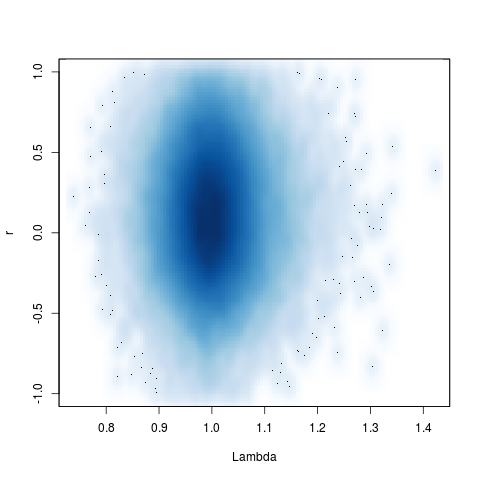
\includegraphics[width=.5\textwidth]{trueLambda.png}
  \caption{\textbf{Effect of the True Lambda of Full Phylogeny.}}
\end{figure}

\begin{figure}[!ht]
  \center
  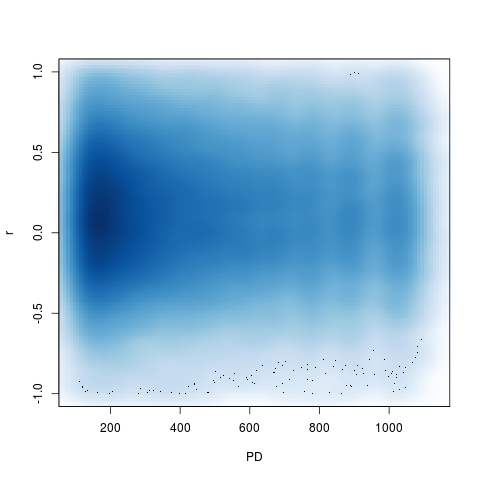
\includegraphics[width=.5\textwidth]{PD.png}
  \caption{\textbf{Effect of True PD of Full Phylogeny.}}
\end{figure}

\begin{figure}[!ht]
  \center
  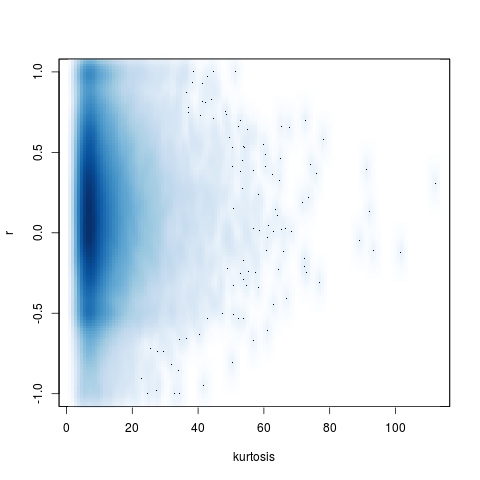
\includegraphics[width=.5\textwidth]{originalKurtosis.png}
  \caption{\textbf{Effect of the True Kurtosis of Full Phylogeny.}}
\end{figure}

\begin{figure}[!ht]
  \center
  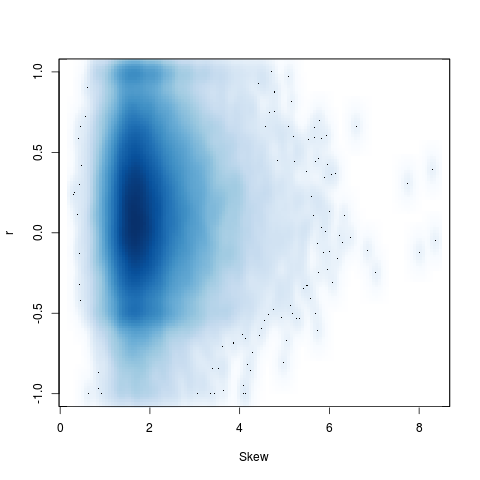
\includegraphics[width=.5\textwidth]{originalSkew.png}
  \caption{\textbf{Effect of the True Skew of Full Phylogeny.}}
\end{figure}

\clearpage
\clearpage
\section*{B. Error Rate in Top Rankings}

\begin{figure}[!ht]
  \center
  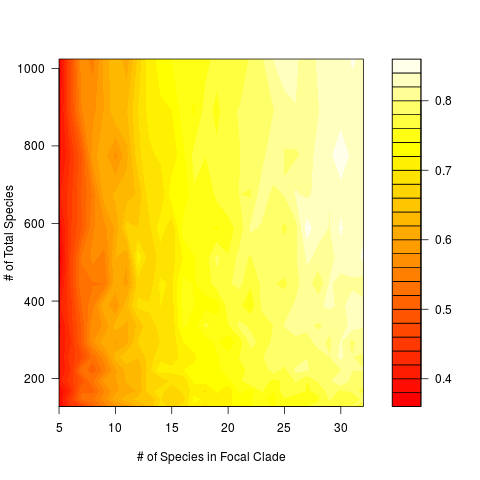
\includegraphics[width=.5\textwidth]{errorRate50.png}
  \caption{\textbf{Mean error rate in the ranking of top 50 species.}}
\end{figure}

\begin{figure}[!ht]
  \center
  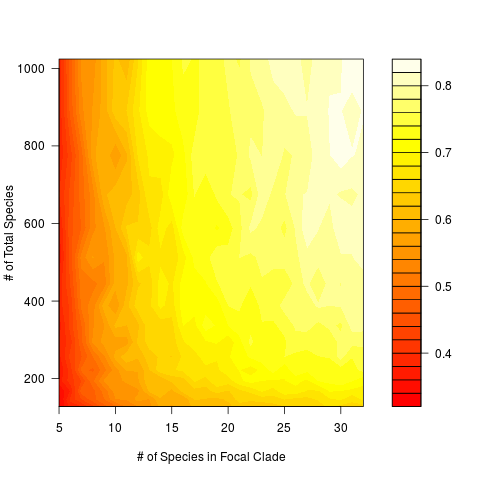
\includegraphics[width=.5\textwidth]{errorRate100.png}
  \caption{\textbf{Mean error rate in the ranking of top 100 species.} }
\end{figure}

\begin{figure}[!ht]
  \center
  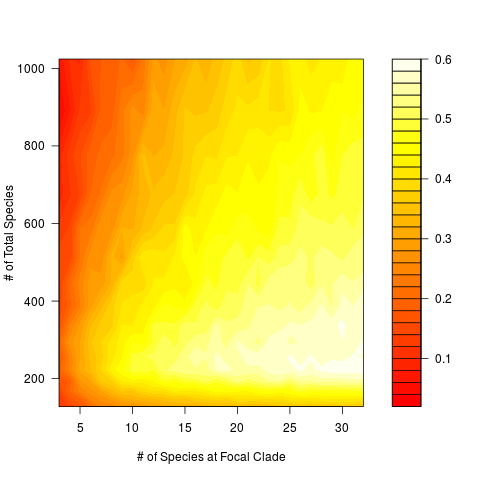
\includegraphics[width=.5\textwidth]{errorRate200.png}
  \caption{\textbf{Mean error rate in the ranking of top 200 species.} }
\end{figure}

\begin{figure}[!ht]
  \center
  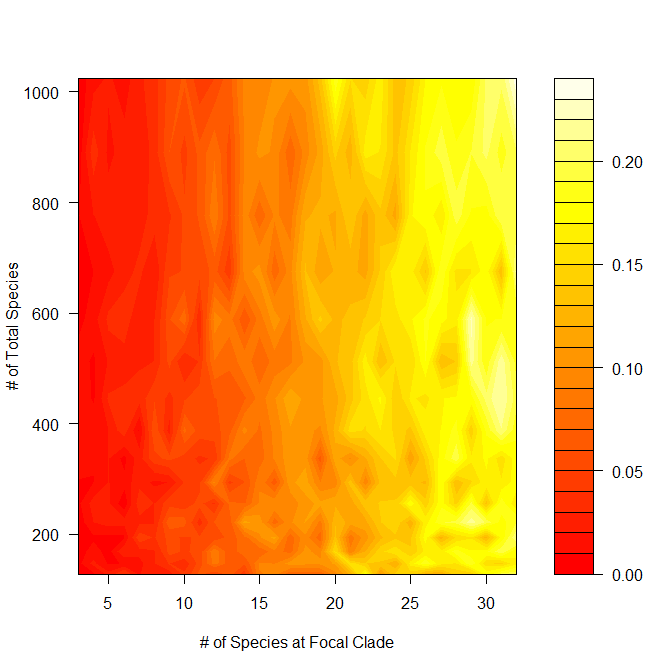
\includegraphics[width=.5\textwidth]{errorRate5pct.png}
  \caption{\textbf{Mean error rate in the ranking of top 5\% of species.} }
\end{figure}

\begin{figure}[!ht]
  \center
  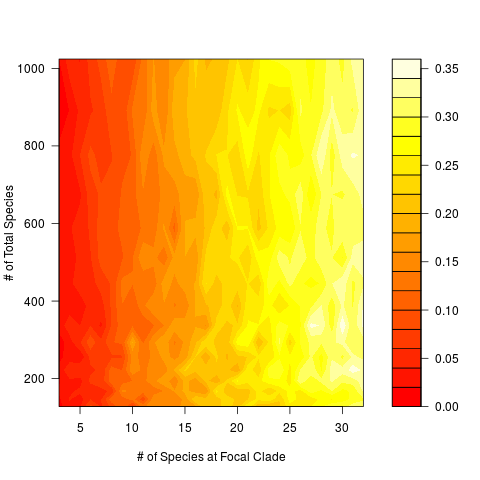
\includegraphics[width=.5\textwidth]{errorRate10pct.png}
  \caption{\textbf{Mean error rate in the ranking of top 10\% of species.} }
\end{figure}

\begin{figure}[!ht]
  \center
  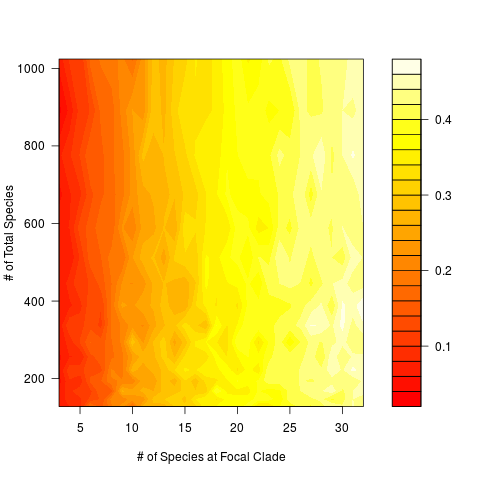
\includegraphics[width=.5\textwidth]{errorRate20pct.png}
  \caption{\textbf{Mean error rate in the ranking of top 20\% of species.}}
\end{figure}

\end{document}
%%% Local Variables:
%%% mode: latex
%%% TeX-master: t
%%% End: